%导演区
\documentclass[a4paper,11pt,UTF8]{article}%book,report,letter
\usepackage[table]{xcolor}
\usepackage{ctex}
\usepackage{geometry}
\geometry{a4paper,scale=0.8}
\usepackage{amsfonts}
\usepackage{amssymb}
\usepackage{verbatim}
\usepackage{mathrsfs}
\usepackage[arrow,matrix]{xy}
\usepackage{amsmath,amssymb,amscd,bm,bbm,amsthm,mathrsfs}
\usepackage{amsmath,amscd}
\usepackage{amsfonts,amssymb}
\usepackage{xypic}
\usepackage{indentfirst}
\usepackage{diagbox}
\usepackage{graphicx}
\usepackage{subfig}    %% 子图包
\usepackage{float} 
\usepackage{caption}
\captionsetup{labelfont=bf}
\usepackage{zhnumber} % change section number to chinese
%这下面为在latex中插入代码所需环境
\usepackage{CJK}
\usepackage{listings}
\usepackage{xcolor}
\lstset{
	language=Matlab,  %代码语言使用的是matlab
	frame=shadowbox, %把代码用带有阴影的框圈起来
	rulesepcolor=\color{red!20!green!20!blue!20},%代码块边框为淡青色
	keywordstyle=\color{blue!90}\bfseries, %代码关键字的颜色为蓝色,粗体
	commentstyle=\color{red!10!green!70}\textit,    % 设置代码注释的颜色
	showstringspaces=false,%不显示代码字符串中间的空格标记
	numbers=left, % 显示行号
	numberstyle=\tiny,    % 行号字体
	stringstyle=\ttfamily, % 代码字符串的特殊格式
	breaklines=true, %对过长的代码自动换行
	extendedchars=false,  %解决代码跨页时,章节标题,页眉等汉字不显示的问题
	texcl=true}
\def\d{\textup{d}}

\theoremstyle{plain}
\newtheorem{thm}{定理}[section]
\newtheorem{lem}{引理}[section]
\newtheorem{prop}{命题}[section]
\newtheorem{cor}{推论}[section]


\renewcommand{\qedsymbol}{$\square$}
\renewcommand\baselinestretch{1.25}
\renewcommand\thesection{\zhnum{section}}
\renewcommand \thesubsection {\arabic{section}}

\usepackage{tabu}                     % 表格插入
\usepackage{multirow}                 % 一般用以设计表格,将所行合并
\usepackage{multicol}                 % 合并多列
\usepackage{multirow}                % 合并多行
\usepackage{float}                    % 图片浮动
\usepackage{makecell}                 % 三线表-竖线
\usepackage{booktabs} 
%正文区
\begin{document}
	\title{\heiti 课题组组会-练习4}
	\author{王程 }
	\date{\today}
	\maketitle
	
	\section{练习及结果}
	1.在$x\in \left[0,1\right]$的均匀网格上尝试使用 Least Squares Recovery(LSR), Least Squares Reconstruction(LSr) 和 Hybrid Least Squares Reconstruction(HLSr) 对$f\left(x\right)$及$g\left(x\right)$进行P1P2重构, 其中$f\left(x\right)=1+x+x^2,g\left(x\right)=sin\left(\pi x\right)$,测试重构精度。如果网格为不均匀网格呢?\\
	\indent 2.在$x\in \left[0,1\right]$的均匀网格上尝试使用 Hybrid Least Squares Reconstruction(HLSr) 对$f\left(x\right)$及$g\left(x\right)$进行 Hyperbolic rDG 的 DG(P0P2)+rDG(P0P1)重构,其中$f\left(x\right)=1+x+x^2+x^3,g\left(x\right)=1+x+x^2+x^3+x^4,h\left(x\right)=sin\left(\pi x\right)$,测试重构精度。 如果网格为不均匀网格呢?\\
	
	\textbf{解:}\\
	\indent(1)分别用三种重构方法对$f\left(x\right)$与$g\left(x\right)$进行P1P2重构,下面展示LSR方法的重构图(非均匀网格):\\
		\begin{figure}[!h]
		\centering
		\subfloat[f重构]{
			\includegraphics[width=3in]{least-squares recovery/f重构.png} 
		}
		\hfill
		\subfloat[g重构]{\includegraphics[width=3in]{least-squares recovery/g重构.png} }
		\caption{LSR}
	\end{figure}\\
\indent LSr与HLSr的重构图与图1类似,这里不重复展示。\\
\clearpage
下面展示不同网格下$f\left(x\right)$与$g\left(x\right)$的精度比较图:\\
		\begin{figure}[!h]
	\centering
	\subfloat[Uniform grid]{
		\includegraphics[width=3in]{比较各个方法的精度/f精度分析(均匀网格).png} 
	}
	\hfill
	\subfloat[Nonuniform grid]{\includegraphics[width=3in]{比较各个方法的精度/f精度分析.png} }
	\caption{f精度分析}
\end{figure}\\
		\begin{figure}[!h]
	\centering
	\subfloat[Uniform grid]{
		\includegraphics[width=3in]{比较各个方法的精度/g精度分析(均匀网格).png} 
	}
	\hfill
	\subfloat[Nonuniform grid]{\includegraphics[width=3in]{比较各个方法的精度/g精度分析.png} }
	\caption{g精度分析}
\end{figure}\\
注意:虽然LSR与HLSr方法下$f\left(x\right)$没有Order,但其误差值达到了机器误差。下述表格能更直观地看出各个方法之间的差别。
\clearpage


\begin{table*}
	\centering
	\caption{非均匀网格下各方法比较}
	\label{tbl:table1}
	\begin{tabular}{cccccccc}
		\Xhline{2pt}
		\multirow{2}{*}{Num of cells} & \multicolumn{2}{c}{P1P2(LSR)} & \multicolumn{2}{c}{P1P2(LSr)} & \multicolumn{2}{c}{P1P2(HLSr)}  \\
			\Xcline{2-3}{0.4pt} 	\Xcline{4-5}{0.4pt} 	\Xcline{6-7}{0.4pt}
		& L2-errors& order &L2-errors& order &L2-errors& order\\
	\Xhline{0.5pt}\\
	case 1: $f\left(x\right)=1+x+x^2$\\
	8& 1.70E-16& & 2.74E-8& &1.56E-16& \\
	16& 2.95E-16&--- & 1.77E-8&3.95 &2.17E-16&--- \\
	32& 4.10E-16&--- & 1.11E-9&3.40 &6.05E-16&--- \\
	64& 1.00E-15&--- & 6.94E-11&4.00 &9.37E-16&--- \\
	\Xhline{0.5pt}\\
	case 2: $g\left(x\right)=sin\left(\pi x\right)$\\
		8& 4.51E-4& & 4.13E-4& &4.53E-4& \\
	16& 4.28E-5&3.40 & 4.06E-5&3.35 &3.96E-5&3.52 \\
	32& 3.81E-6&3.49 & 3.68E-6&3.46 &3.48E-6&3.50 \\
	64& 3.57E-7&3.41& 3.37E-7&3.45 &3.42E-7&3.35 \\
	\Xhline{2pt}
\end{tabular} 
\end{table*}
~\\
\indent(2)在$x\in \left[0,1\right]$上使用 Hybrid Least Squares Reconstruction(HLSr) 对$f\left(x\right)$及$g\left(x\right)$与进行$h\left(x\right)$ Hyperbolic rDG 的 DG(P0P2)+rDG(P0P1)重构,分别对$\varphi$和$v$选取方程进行重构求解,最终得到如下结果(仅考虑非均匀网格,均匀网格视为非均匀网格的一个特例):\\
~\\
\textbf{A)}$f\left(x\right)=x^3+x^2+x+1$
	\begin{figure}[!h]
	\centering
	\subfloat[重构图]{
		\includegraphics[width=3in]{Hyperbolic rDG HLSr/f重构.png} 
	}
	\hfill
	\subfloat[精度分析]{\includegraphics[width=3in]{Hyperbolic rDG HLSr/f精度分析.png} }
	\caption{f(x)}
\end{figure}\\
\clearpage
\noindent \textbf{B)}$g\left(x\right)=x^4+x^3+x^2+x+1$
\begin{figure}[!h]
	\centering
	\subfloat[重构图]{
		\includegraphics[width=3in]{Hyperbolic rDG HLSr/g重构.png} 
	}
	\hfill
	\subfloat[精度分析]{\includegraphics[width=3in]{Hyperbolic rDG HLSr/g精度分析.png} }
	\caption{g(x)}
\end{figure}\\
\textbf{C)}$h\left(x\right)=sin\left(\pi x\right)$
\begin{figure}[!h]
	\centering
	\subfloat[重构图]{
		\includegraphics[width=3in]{Hyperbolic rDG HLSr/h重构.png} 
	}
	\hfill
	\subfloat[精度分析]{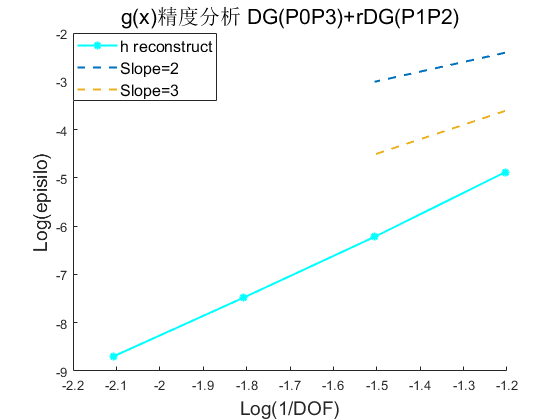
\includegraphics[width=3in]{Hyperbolic rDG HLSr/h精度分析.png} }
	\caption{h(x)}
\end{figure}\\

	\clearpage
	\section{附录(代码,仅展示部分)}
	\noindent \textbf{LSR}
	\lstset{language=Matlab}%代码语言使用的是matlab
	\lstset{breaklines}%自动将长的代码行换行排版
	\lstset{extendedchars=false}%解决代码跨页时,章节标题,页眉等汉字不显示的问题
\begin{lstlisting}
clc
clear all
close all
%% Pre-proceeding
Unit=8;endx=1;deltax=endx/Unit;numberx=Unit+1;
%记录内点位置,上下浮动不超过百分之5
Grid=zeros(1,numberx);
for i=2:numberx-1
Grid(1,i)=(i-1)*deltax+(0.1*rand(1)-0.05)*deltax;
end
Grid(1,numberx)=endx;
f=@(x)x.^2+x+1;F=@(x)2*x+1;
g=@(y)sin(pi*y);G=@(y)pi*cos(pi*y);
Unumsolution=zeros(2,Unit);
Ureconstruct=zeros(1,Unit);
Unumsolution1=zeros(1,2);
Unumsolution2=zeros(2,numberx-1);
Acc=zeros(3,4);a1=[1/8,1/16,1/32,1/64];a2=[1/8,1/16];
%% Proceeding
%对f
for k=1:Unit
Unumsolution(1,k)=(Grid(k+1)-Grid(k)+0.5*(Grid(k+1)^2-Grid(k)^2)+(Grid(k+1)^3-Grid(k)^3)/3)/(Grid(k+1)-Grid(k));
Unumsolution(2,k)=F(0.5*(Grid(k)+Grid(k+1)))*(Grid(k+1)-Grid(k));%store Uxc*deltax
end
		
%Reconstruct Uxx
for k=2:numberx-2
xci=0.5*(Grid(k)+Grid(k+1));%xci
xci1=0.5*(Grid(k+1)+Grid(k+2));%xci+1
xci2=0.5*(Grid(k-1)+Grid(k));%xci-1
A=[(xci1-xci)^2/(2*(Grid(k+1)-Grid(k))^2)+1/24*((Grid(k+2)-Grid(k+1))^2/(Grid(k+1)-Grid(k))^2-1);
(Grid(k+2)-Grid(k+1))*(xci1-xci)/(Grid(k+1)-Grid(k))^2;
(xci2-xci)^2/(2*(Grid(k+1)-Grid(k))^2)+1/24*((Grid(k)-Grid(k-1))^2/(Grid(k+1)-Grid(k))^2-1);
(Grid(k)-Grid(k-1))*(xci2-xci)/(Grid(k+1)-Grid(k))^2];
b=[Unumsolution(1,k+1)-Unumsolution(1,k)-Unumsolution(2,k)*(xci1-xci)/(Grid(k+1)-Grid(k));
Unumsolution(2,k+1)-Unumsolution(2,k)*(Grid(k+2)-Grid(k+1))/(Grid(k+1)-Grid(k));
Unumsolution(1,k-1)-Unumsolution(1,k)-Unumsolution(2,k)*(xci2-xci)/(Grid(k+1)-Grid(k));
Unumsolution(2,k-1)-Unumsolution(2,k)*(Grid(k)-Grid(k-1))/(Grid(k+1)-Grid(k))];
Ureconstruct(k)=A\b;
end
%boundary
%Left
xci=0.5*(Grid(1)+Grid(2));%xci
xci1=0.5*(Grid(2)+Grid(3));%xci+1
A=[(xci1-xci)^2/(2*(Grid(2)-Grid(1))^2)+1/24*((Grid(3)-Grid(2))^2/(Grid(2)-Grid(1))^2-1);
(Grid(3)-Grid(2))*(xci1-xci)/(Grid(2)-Grid(1))^2];
b=[Unumsolution(1,2)-Unumsolution(1,1)-Unumsolution(2,1)*(xci1-xci)/(Grid(2)-Grid(1));
Unumsolution(2,2)-Unumsolution(2,1)*(Grid(3)-Grid(2))/(Grid(2)-Grid(1))];    
Ureconstruct(1)=A\b;
%Right    
xci=0.5*(Grid(numberx-1)+Grid(numberx-1+1));%xci
xci2=0.5*(Grid(numberx-1-1)+Grid(numberx-1));%xci-1    
A=[(xci2-xci)^2/(2*(Grid(numberx-1+1)-Grid(numberx-1))^2)+1/24*((Grid(numberx-1)-Grid(numberx-1-1))^2/(Grid(numberx-1+1)-Grid(numberx-1))^2-1);
(Grid(numberx-1)-Grid(numberx-1-1))*(xci2-xci)/(Grid(numberx-1+1)-Grid(numberx-1))^2];
b=[Unumsolution(1,numberx-1-1)-Unumsolution(1,numberx-1)-Unumsolution(2,numberx-1)*(xci2-xci)/(Grid(numberx-1+1)-Grid(numberx-1));
Unumsolution(2,numberx-1-1)-Unumsolution(2,numberx-1)*(Grid(numberx-1)-Grid(numberx-1-1))/(Grid(numberx-1+1)-Grid(numberx-1))];   
Ureconstruct(numberx-1)=A\b;
		
%Post-proceeding
figure
k=1;
x=Grid(k):0.2*(Grid(k+1)-Grid(k)):Grid(k+1);
p=[Ureconstruct(k)/(2*(Grid(k+1)-Grid(k))^2),Unumsolution(2,k)/(Grid(k+1)-Grid(k))-Ureconstruct(k)*0.5*(Grid(k+1)+Grid(k))/(Grid(k+1)-Grid(k))^2,Unumsolution(1,k)+Ureconstruct(k)*(0.5*(Grid(k+1)+Grid(k)))^2/(2*(Grid(k+1)-Grid(k))^2)-Unumsolution(2,k)*0.5*(Grid(k+1)+Grid(k))/(Grid(k+1)-Grid(k))-Ureconstruct(k)/24];
y=polyval(p,x);
plot(x,y,'-r^','linewidth',1.5);hold on
H1=plot(x,y,'-r^','linewidth',1.5);hold on
		
for k=2:numberx-1
x=Grid(k):0.2*(Grid(k+1)-Grid(k)):Grid(k+1);
p=[Ureconstruct(k)/(2*(Grid(k+1)-Grid(k))^2),Unumsolution(2,k)/(Grid(k+1)-Grid(k))-Ureconstruct(k)*0.5*(Grid(k+1)+Grid(k))/(Grid(k+1)-Grid(k))^2,Unumsolution(1,k)+Ureconstruct(k)*(0.5*(Grid(k+1)+Grid(k)))^2/(2*(Grid(k+1)-Grid(k))^2)-Unumsolution(2,k)*0.5*(Grid(k+1)+Grid(k))/(Grid(k+1)-Grid(k))-Ureconstruct(k)/24];
y=polyval(p,x);plot(x,y,'-r^','linewidth',1.5);
end
		
hold on
x=Grid(1):0.01*(Grid(numberx)-Grid(1)):Grid(numberx);
plot(x,f(x),'-b','linewidth',1.5);
H2=plot(x,f(x),'-b','linewidth',1.5);
lgd=legend([H1,H2],'Reconstruct','Exact solution');
lgd.FontSize=12;
xlabel('位置x','fontsize',14)
ylabel('数值U','fontsize',14)
title('Nonuniform grid reconstruct f=x^2+x+1','fontsize',16)
hold off
		
%计算精度
Acc(1,1)=Accuracy(8);Acc(1,2)=Accuracy(16);
Acc(1,3)=Accuracy(32);
Acc(1,4)=Accuracy(64);
for k=1:3
accuracyf(k)=(log10(Acc(1,k+1))-log10(Acc(1,k)))./(log10(a1(1,k+1))-log10(a1(1,k)));
end
figure
hold on
plot(log10(a1),log10(Acc(1,:)),'-c*','linewidth',1.5)
H1=plot(log10(a1),log10(Acc(1,:)),'-c*','linewidth',1.5);
		
H2=plot(log10(a2),1*log10(a2),'--','linewidth',1.5);
plot(log10(a2),2*log10(a2),'--','linewidth',1.5)
H3=plot(log10(a2),2*log10(a2),'--','linewidth',1.5);
lgd=legend([H1,H2,H3],'f reconstruct','斜率为1','斜率为2');
lgd.FontSize=12;
xlabel('Log(deltax)','fontsize',14)
ylabel('Log(episilo)','fontsize',14)
title('f精度分析','fontsize',16)
		
%对g
for k=1:Unit
Unumsolution(1,k)=(cos(pi*Grid(k))-cos(pi*Grid(k+1)))/(pi*(Grid(k+1)-Grid(k)));
Unumsolution(2,k)=G(0.5*(Grid(k)+Grid(k+1)))*(Grid(k+1)-Grid(k));%store Uxc*deltax
end
		
%Reconstruct Uxx
for k=2:numberx-2	
xci=0.5*(Grid(k)+Grid(k+1));%xci
xci1=0.5*(Grid(k+1)+Grid(k+2));%xci+1
xci2=0.5*(Grid(k-1)+Grid(k));%xci-1
A=[(xci1-xci)^2/(2*(Grid(k+1)-Grid(k))^2)+1/24*((Grid(k+2)-Grid(k+1))^2/(Grid(k+1)-Grid(k))^2-1);
(Grid(k+2)-Grid(k+1))*(xci1-xci)/(Grid(k+1)-Grid(k))^2;
(xci2-xci)^2/(2*(Grid(k+1)-Grid(k))^2)+1/24*((Grid(k)-Grid(k-1))^2/(Grid(k+1)-Grid(k))^2-1);
(Grid(k)-Grid(k-1))*(xci2-xci)/(Grid(k+1)-Grid(k))^2];
b=[Unumsolution(1,k+1)-Unumsolution(1,k)-Unumsolution(2,k)*(xci1-xci)/(Grid(k+1)-Grid(k));
Unumsolution(2,k+1)-Unumsolution(2,k)*(Grid(k+2)-Grid(k+1))/(Grid(k+1)-Grid(k));
Unumsolution(1,k-1)-Unumsolution(1,k)-Unumsolution(2,k)*(xci2-xci)/(Grid(k+1)-Grid(k));
Unumsolution(2,k-1)-Unumsolution(2,k)*(Grid(k)-Grid(k-1))/(Grid(k+1)-Grid(k))];
Ureconstruct(k)=A\b;
end
%boundary
%Left
xci=0.5*(Grid(1)+Grid(2));%xci
xci1=0.5*(Grid(2)+Grid(3));%xci+1
A=[(xci1-xci)^2/(2*(Grid(2)-Grid(1))^2)+1/24*((Grid(3)-Grid(2))^2/(Grid(2)-Grid(1))^2-1);
(Grid(3)-Grid(2))*(xci1-xci)/(Grid(2)-Grid(1))^2];
b=[Unumsolution(1,2)-Unumsolution(1,1)-Unumsolution(2,1)*(xci1-xci)/(Grid(2)-Grid(1));
Unumsolution(2,2)-Unumsolution(2,1)*(Grid(3)-Grid(2))/(Grid(2)-Grid(1))];    
Ureconstruct(1)=A\b;
%Right    
xci=0.5*(Grid(numberx-1)+Grid(numberx-1+1));%xci
xci2=0.5*(Grid(numberx-1-1)+Grid(numberx-1));%xci-1    
A=[(xci2-xci)^2/(2*(Grid(numberx-1+1)-Grid(numberx-1))^2)+1/24*((Grid(numberx-1)-Grid(numberx-1-1))^2/(Grid(numberx-1+1)-Grid(numberx-1))^2-1);
(Grid(numberx-1)-Grid(numberx-1-1))*(xci2-xci)/(Grid(numberx-1+1)-Grid(numberx-1))^2];
b=[Unumsolution(1,numberx-1-1)-Unumsolution(1,numberx-1)-Unumsolution(2,numberx-1)*(xci2-xci)/(Grid(numberx-1+1)-Grid(numberx-1));
Unumsolution(2,numberx-1-1)-Unumsolution(2,numberx-1)*(Grid(numberx-1)-Grid(numberx-1-1))/(Grid(numberx-1+1)-Grid(numberx-1))];   
Ureconstruct(numberx-1)=A\b;
%Post-proceeding
figure
k=1;
x=Grid(k):0.2*(Grid(k+1)-Grid(k)):Grid(k+1);
p=[Ureconstruct(k)/(2*(Grid(k+1)-Grid(k))^2),Unumsolution(2,k)/(Grid(k+1)-Grid(k))-Ureconstruct(k)*0.5*(Grid(k+1)+Grid(k))/(Grid(k+1)-Grid(k))^2,Unumsolution(1,k)+Ureconstruct(k)*(0.5*(Grid(k+1)+Grid(k)))^2/(2*(Grid(k+1)-Grid(k))^2)-Unumsolution(2,k)*0.5*(Grid(k+1)+Grid(k))/(Grid(k+1)-Grid(k))-Ureconstruct(k)/24];
y=polyval(p,x);
plot(x,y,'-ro','linewidth',1.5);hold on
H1=plot(x,y,'-ro','linewidth',1.5);hold on
		
for k=2:numberx-1
x=Grid(k):0.2*(Grid(k+1)-Grid(k)):Grid(k+1);
p=[Ureconstruct(k)/(2*(Grid(k+1)-Grid(k))^2),Unumsolution(2,k)/(Grid(k+1)-Grid(k))-Ureconstruct(k)*0.5*(Grid(k+1)+Grid(k))/(Grid(k+1)-Grid(k))^2,Unumsolution(1,k)+Ureconstruct(k)*(0.5*(Grid(k+1)+Grid(k)))^2/(2*(Grid(k+1)-Grid(k))^2)-Unumsolution(2,k)*0.5*(Grid(k+1)+Grid(k))/(Grid(k+1)-Grid(k))-Ureconstruct(k)/24];
y=polyval(p,x);
plot(x,y,'-ro','linewidth',1.5);
end
hold on
x=Grid(1):0.01*(Grid(numberx)-Grid(1)):Grid(numberx);
plot(x,g(x),'-b','linewidth',1.5);
H2=plot(x,g(x),'-b','linewidth',1.5);
lgd=legend([H1,H2],'Reconstruct','Exact solution');
lgd.FontSize=12;
xlabel('位置x','fontsize',14)
ylabel('数值U','fontsize',14)
title('Nonuniform grid reconstruct g=sin(pi*x) ','fontsize',16)
hold off
		
%计算精度
Acc(1,1)=Accuracyg(8);
Acc(1,2)=Accuracyg(16);
Acc(1,3)=Accuracyg(32);
Acc(1,4)=Accuracyg(64);
for k=1:3
accuracyg(k)=(log10(Acc(1,k+1))-log10(Acc(1,k)))./(log10(a1(1,k+1))-log10(a1(1,k)));
end
figure
hold on
plot(log10(a1),log10(Acc(1,:)),'-c*','linewidth',1.5)
H1=plot(log10(a1),log10(Acc(1,:)),'-c*','linewidth',1.5);
H2=plot(log10(a2),1*log10(a2),'--','linewidth',1.5);
plot(log10(a2),2*log10(a2),'--','linewidth',1.5)
H3=plot(log10(a2),2*log10(a2),'--','linewidth',1.5);
lgd=legend([H1,H2,H3],'g reconstruct','斜率为1','斜率为2');
lgd.FontSize=12;
xlabel('Log(deltax)','fontsize',14)
ylabel('Log(episilo)','fontsize',14)
title('g精度分析','fontsize',16)	
\end{lstlisting}
	

\end{document}